\section{Tarea}

Este proyecto tiene por objetivo que los alumnos implementen un sistema de detección de
plagio simple (sistema a ser implementado), en el cual, usando como referencia una base
de datos, el usuario del sistema enviará un párrafo escrito por el mismo (o copiado de
alguna fuente) y lo enviará al sistema, el cual se encarga de realizar las consultas sobre la base de datos a fin de determinar si existió plagio o no.
\subsection*{Consideraciones importantes}
\begin{enumerate}
    \item \textbf{Eficiencia del sistema:} En general, los sistemas priman la eficiencia y la velocidad con la que realizan sus funcionalidades, y en este proyecto no podíamos dejar de lado esto Garantizar velocidad en detectores de plagio muchas veces requiere que se realicen
pre-procesamientos sobre los textos, a fin de reducir la cantidad de contenido a ser
consultado.\\

\textbf{Pre-procesamientos} comunes incluyen: eliminación de caracteres especiales (por
ejemplo, puntos, comas, parentesis, etc.), extracción de raíces de las palabras (por
ejemplo, “act-” sería la raíz de las palabras “actor”, “actores”, “actriz”, etc.), etc. Estos
pre-procesamientos reducen considerablemente la complejidad de la búsqueda de
coincidencias, pues son menos comparaciones a ser realizadas.\\

Sin embargo, el uso de pre-procesamientos algunas veces impactan en la eficiencia
de la detección de plagio, pues se pierde la comparación exacta de palabras y
frases.
    \item  \textbf{Número de integrantes:} Este proyecto será realizado en grupos entre 3 y 4
integrantes. Cada grupo tendrá un líder, el cual debe enviar en las fechas
correspondientes los diferentes entregables solicitados por los profesores.

\end{enumerate}
\section{URL de Repositorio Github}
\begin{itemize}
    \item URL del Repositorio GitHub para clonar o recuperar.
    \item \url{https://github.com/MaxsForocca/Lab_EDA_PlagiarismDetector.git}
\end{itemize}


% \section{Ejecuciones}
\section{Implementacion del codigo}


\subsection{Clase \texttt{NodeTrie}}
Esta clase representa un nodo en la estructura de datos Trie.

\textbf{Atributos:}
\begin{itemize}
    \item \texttt{NodeTrie[] children}: Arreglo de nodos hijos que representa las letras del alfabeto.
    \item \texttt{boolean isWord}: Indica si el nodo actual marca el final de una palabra.
\end{itemize}

\textbf{Métodos:}
\begin{itemize}
    \item \texttt{NodeTrie()}: Constructor que inicializa el arreglo de nodos hijos y establece \texttt{isWord} como falso.
    \item \texttt{getChildren()}: Retorna el arreglo de nodos hijos.
    \item \texttt{isAWord()}: Devuelve \texttt{true} si el nodo actual marca el final de una palabra.
    \item \texttt{setIsWord(boolean isWord)}: Establece el indicador \texttt{isWord} para marcar si el nodo forma una palabra.
    \item \texttt{getChild(char c)}: Retorna el nodo hijo correspondiente a la letra \texttt{c}.
    \item \texttt{setChild(char c, NodeTrie child)}: Establece el nodo hijo \texttt{child} correspondiente a la letra \texttt{c}.
\end{itemize}

\lstinputlisting[language=java,numbers=left,]{src/NodeTrie.java}

\subsection{Clase \texttt{Trie}}
Esta clase representa la estructura de datos Trie que almacena palabras y permite búsquedas eficientes.

\textbf{Atributos:}
\begin{itemize}
    \item \texttt{NodeTrie root}: El nodo raíz del Trie.
\end{itemize}

\textbf{Métodos:}
\begin{itemize}
    \item \texttt{Trie()}: Constructor que inicializa la estructura Trie creando un nodo raíz.
    \item \texttt{insert(String word)}: Inserta una palabra en el Trie, creando nodos hijos según las letras de la palabra.
    \item \texttt{search(String word)}: Realiza una búsqueda en el Trie para verificar si una palabra existe en él.
\end{itemize}

\lstinputlisting[language=java,numbers=left,]{src/Trie.java}

\subsection{Clase \texttt{PlagiarismDetector}}
Esta clase se encarga de cargar los archivos de texto, construir los tries y realizar la detección de plagio utilizando la estructura Trie.

\textbf{Atributos:}
\begin{itemize}
    \item \texttt{static String folderPath}: Ruta de la carpeta que contiene los archivos de texto.
    \item \texttt{static File[] files}: Arreglo que almacena los archivos de texto en la carpeta.
    \item \texttt{static ArrayList<Trie> tries}: Lista de objetos Trie para almacenar las palabras de los archivos.
\end{itemize}

\textbf{Métodos:}
\begin{itemize}
    \item \texttt{main(String[] args)}: Punto de entrada del programa que carga los archivos, construye los tries y realiza la detección de plagio.
    \item \texttt{loadFiles(File[] files)}: Carga los archivos de texto, procesa las palabras y crea los objetos Trie correspondientes.
    \item  \texttt{procesarTexto(String str)}: Realiza un procesamiento de texto, quitando los caracteres con tildes o cambiando la 'ñ' por la 'n', retorna un arreglo de las palabras ya procesadas de la cadena str.
    \item \texttt{detectarPlagioPalabras(String texto)}: Realiza la detección de plagio para un texto ingresado, calculando el porcentaje de similitud con los tries almacenados.
    \item \texttt{verifyPlagiarism(String path)}: Método por implementar para verificar los resultados de la detección de plagio.
\end{itemize}

Esta clase en general busca determinar el porcentaje de similitud entre el texto ingresado y los archivos de texto previamente cargados en los tries. Cada trie se utiliza para verificar la presencia de palabras del texto ingresado en los archivos almacenados, calculando el porcentaje de coincidencia en relación al total de palabras en el texto.

\lstinputlisting[language=java,numbers=left,]{src/PlagiarismDetector.java}
\subsection{Clase \texttt{Vista}}
Esta clase se encarga realizar la interfaz gráfica de usuario GUI. Que utiliza la librería swing.

\textbf{Atributos:}
\begin{itemize}
    \item \texttt{javax.swing.JButton btnCom, btnSel, btnSel2}: Botones de la interfaz.
    \item  \texttt{javax.swing.JLabel jLabel1, jLabel2, jLabel3, jLabel4, jLabel5, jLabel6, jLabel7, lbPT}: Etiquetas de texto de la interfaz.
    \item  \texttt{javax.swing.JPanel jPanel1}: Contenedor para los componentes de la interfaz.
    \item  \texttt{javax.swing.JScrollPane jScrollPane1, jScrollPane2}: Barras de desplazamiento para componentes de la interfaz.
    \item  \texttt{javax.swing.JTextArea txaArchivo, txaArchivo2}: Áreas de texto de la interfaz.
\end{itemize}

\textbf{Métodos:}
\begin{itemize}
    \item \texttt{Vista()}: Constructor que llama al método "initComponents()" y establece la ubicación de la ventana en el centro de la pantalla.
    \item  \texttt{btnSelActionPerformed(java.awt.event.ActionEvent evt)}: Este método maneja los eventos del botón 'subir' y crea un cuadro de selección de archivos usando JFileChooser, el archivo seleccionado se lee mediante FileReader y BufferedReader, y su contenido se muestra en la primera área de texto mediante el método "setText()".
    \item \texttt{btnSel2ActionPerformed(java.awt.event.ActionEvent evt)}: Lo mismo que el anterior.
    \item \texttt{main(String args[])}: El metodo principal que se encarga de configurar el aspecto visual de la aplicación y de crear y mostrar la ventana de la GUI.
\end{itemize}\clearpage
\section{Vistas}

\begin{figure}[h!]
    \centering
    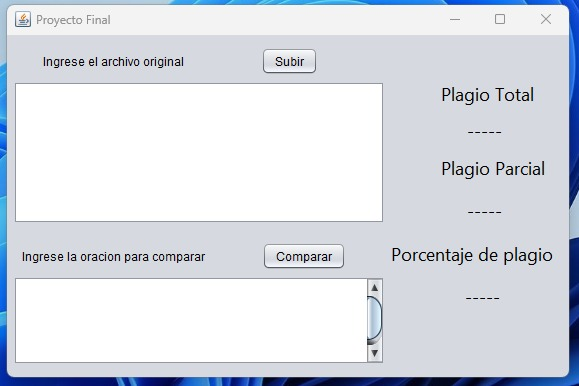
\includegraphics[scale=0.6]{img/caos.jpeg}
\end{figure}


\section{Referencias}

\begin{itemize}
    \item https://www.geeksforgeeks.org/trie-insert-and-search/
    \item https://www.baeldung.com/trie-java
    \item https://www.techiedelight.com/es/implement-trie-data-structure-java/
\end{itemize}

